\subsection{\texorpdfstring{W+jets Background Estimation in $\tauTau$ Channel}{W+jets Background Estimation in tau-tau Channel}}
\subsubsection{Method Description}
As shown in the cut-flow-table, the number of W+jets events surviving the selection cuts are found to be zero in search \binone or 0.43$\pm$0.40 in search \bintwo. In other words, due to the low statistics of W+jets events, the efficiency of $\mttwo$ is obtained to be zero, in \binone, or as found in \bintwo, the efficiency of $\SumMT$ is obtained very close to zero with a huge statistical uncertainty, namely 93\%. The statistical uncertainty on the yields for W+jets events can be improved by extracting the $\mttwo$ or $\SumMT$ cut efficieny, depending on the serach bins, in a sample with more statistics. This region is defined by relaxing some cuts which have marginal effects on either $\mttwo$ or $\SumMT$ variables. This way, the yields for W+jets events are reported with more statistical accuracy. In the next subsection, the validation of this method will be discussed.\\

\subsubsection{Method Validation}
Figure~\ref{fig:justification_bin1}  
\begin{figure}[htbp]
\centering
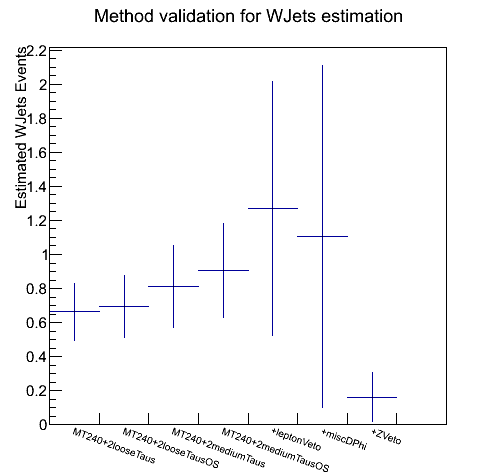
\includegraphics[angle=0,scale=0.35]{TauTauFigs/withMT2GT40.png}
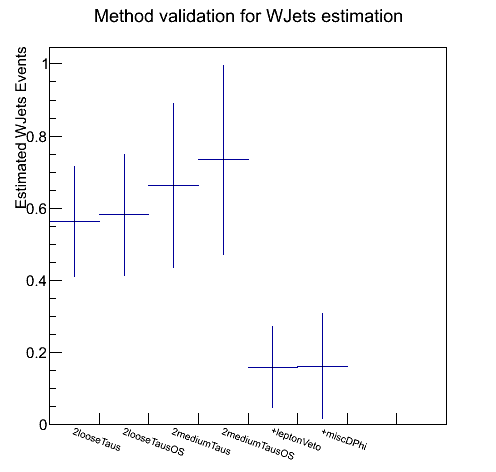
\includegraphics[angle=0,scale=0.35]{TauTauFigs/withMT2GT40ZVeto.png} \\
\caption{Cut efficiency for $\mttwo$ %(left) and \SumMT (right) 
in samples with various selections as labeled in each bin.}
\label{fig:justification_bin1}
\end{figure}
Figure~\ref{fig:justification_bin2}  
\begin{figure}[htbp]
\centering
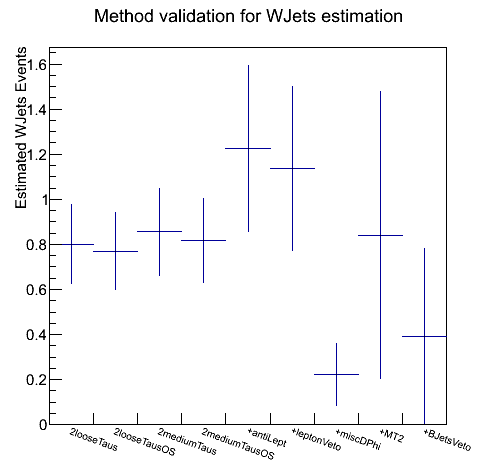
\includegraphics[angle=0,scale=0.35]{TauTauFigs/WJetsEst_bin2.png}
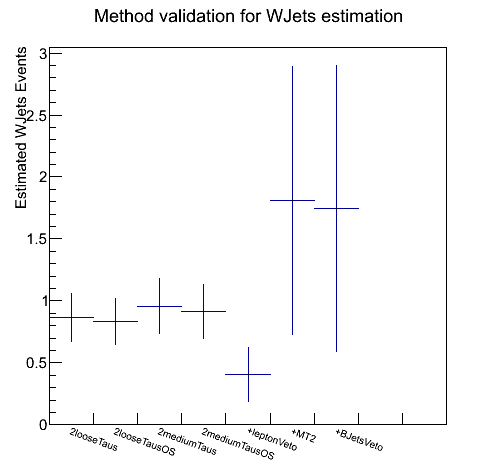
\includegraphics[angle=0,scale=0.35]{TauTauFigs/WJetsEst_bin2_miscApplied.png} \\
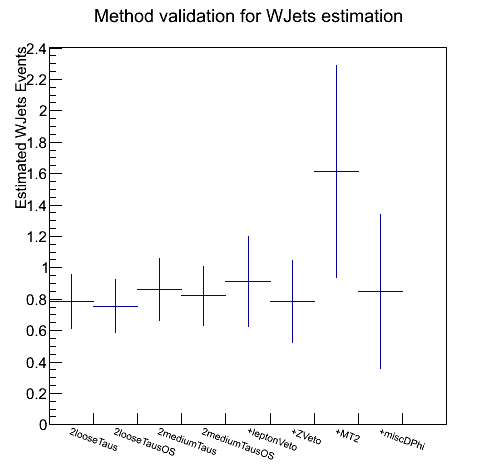
\includegraphics[angle=0,scale=0.35]{TauTauFigs/WJetsEst_bin2_BJetVetoApplied.png} \\
\caption{Cut efficiency for %\mttwo (left) and 
$\SumMT$ %(right) 
in samples with various selections as labeled in each bin.}
\label{fig:justification_bin2}
\end{figure}


